\section{Simulazioni modello di Ising 1D}

\begin{figure}[H]
    \centering
    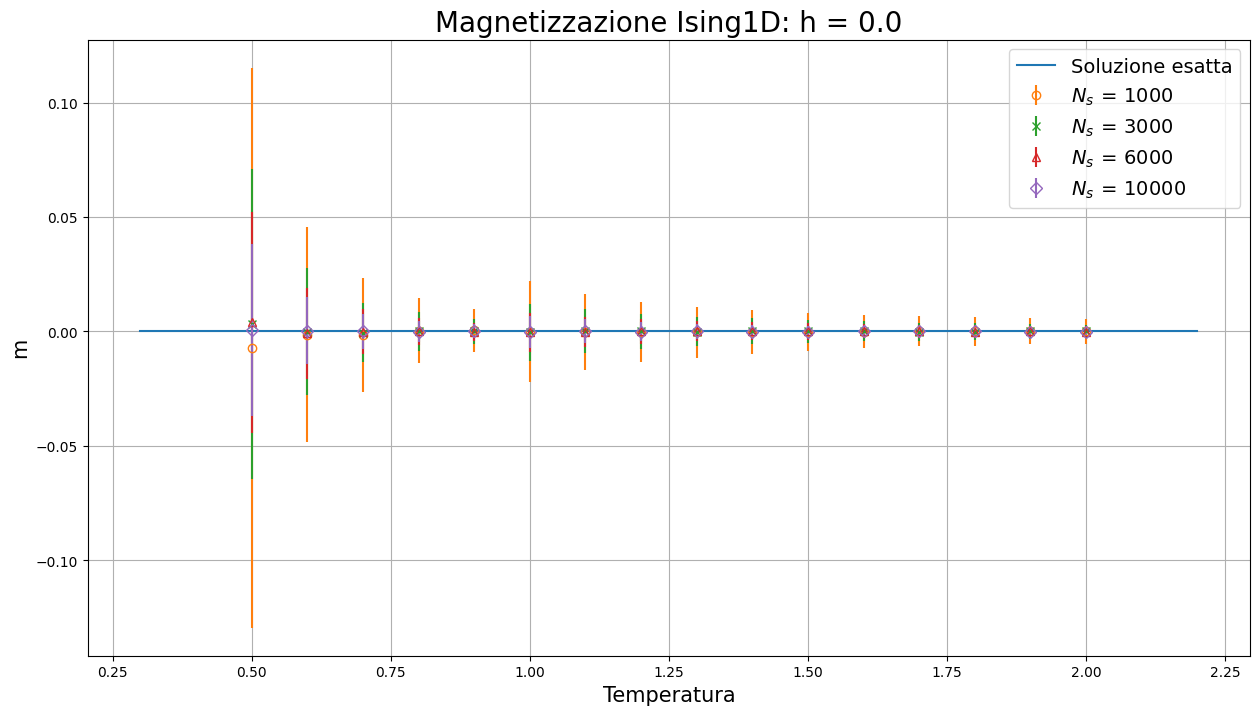
\includegraphics[width=\textwidth]{Immagini/simIsing1D/magn_h0.0.png}
    \caption{Magnetizzazione modello di Ising 1D: h = 0.0.}
    \label{fig: magn_Ising1D_h0.0}
\end{figure}

\begin{figure}[H]
    \centering
    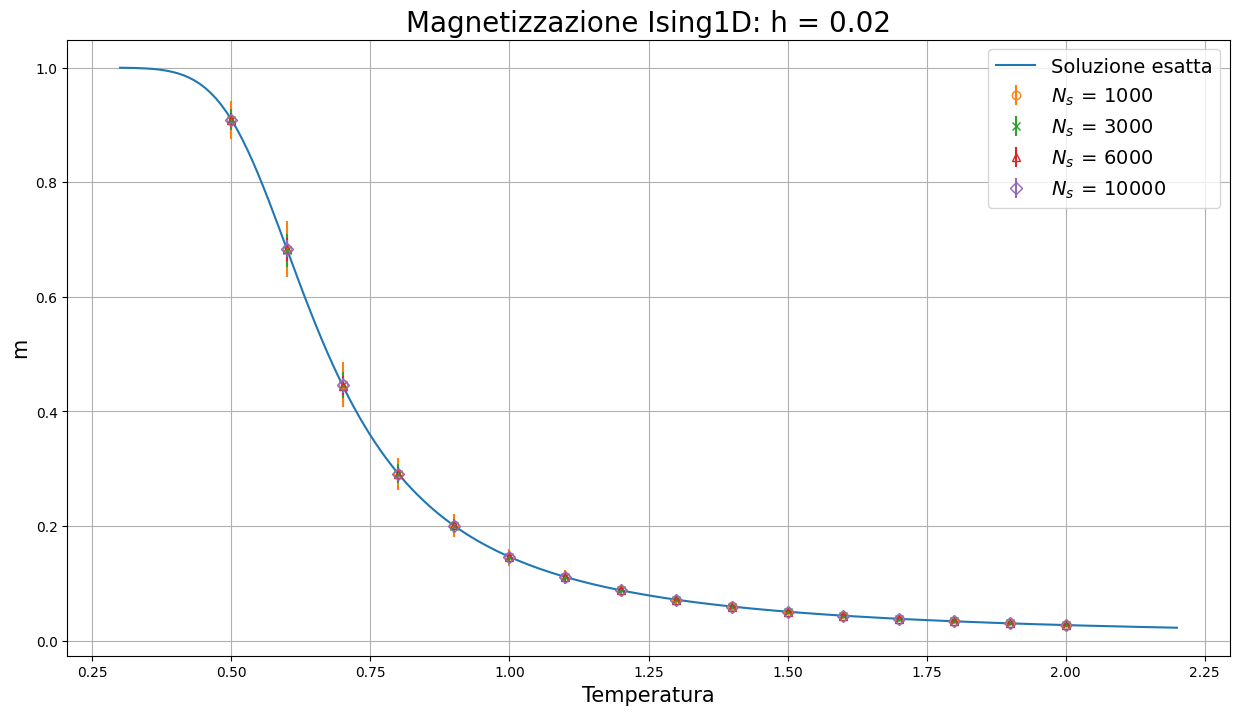
\includegraphics[width=\textwidth]{Immagini/simIsing1D/magn_h0.02.png}
    \caption{Magnetizzazione modello di Ising 1D: h = 0.02.}
    \label{fig: magn_Ising1D_h0.02}
\end{figure}

\begin{figure}[H]
    \centering
    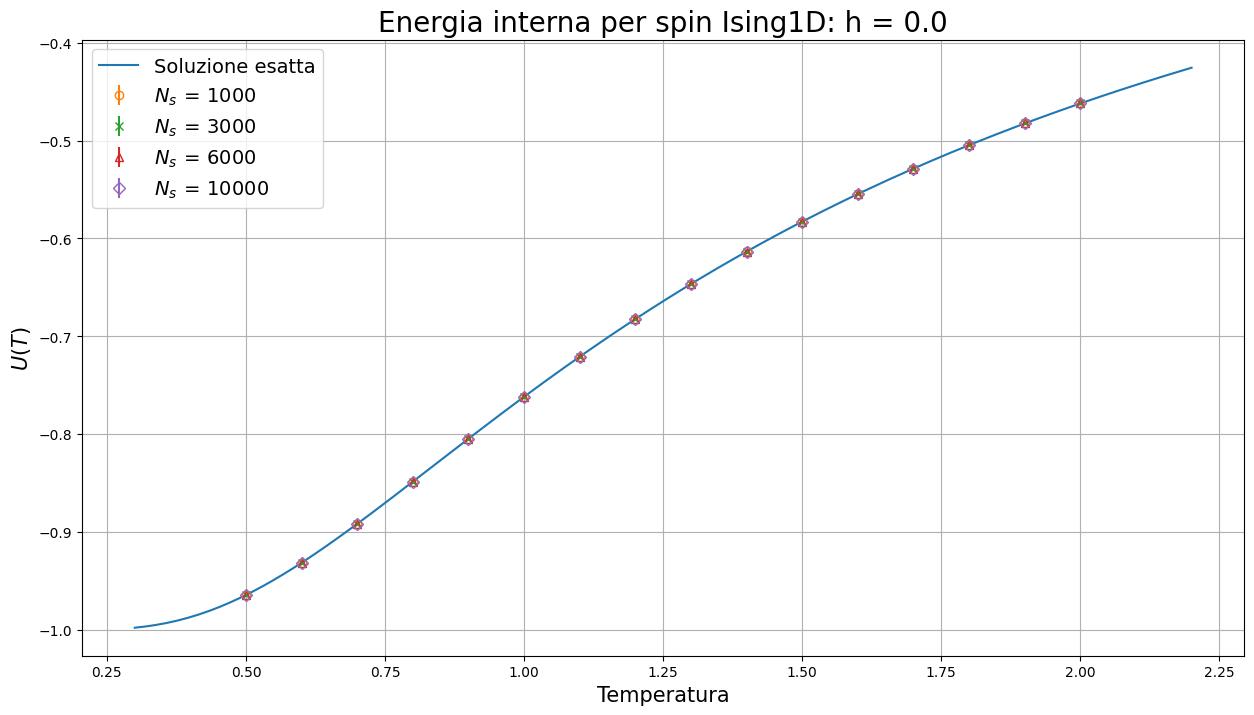
\includegraphics[width=\textwidth]{Immagini/simIsing1D/ene_h0.0.png}
    \caption{Energia modello di Ising 1D: h = 0.0.}
    \label{fig: ene_Ising1D_h0.0}
\end{figure}

\begin{figure}[H]
    \centering
    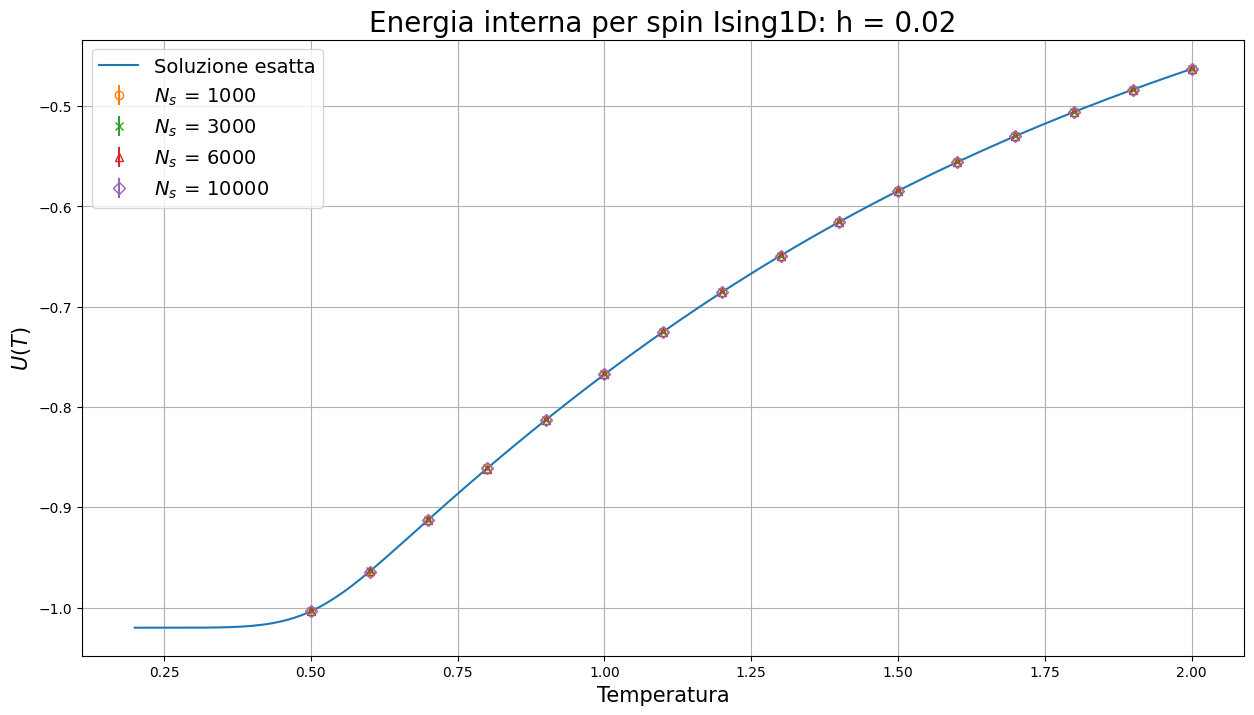
\includegraphics[width=\textwidth]{Immagini/simIsing1D/ene_h0.02.png}
    \caption{Energia modello di Ising 1D: h = 0.02.}
    \label{fig: ene_Ising1D_h0.02}
\end{figure}

\begin{figure}[H]
    \centering
    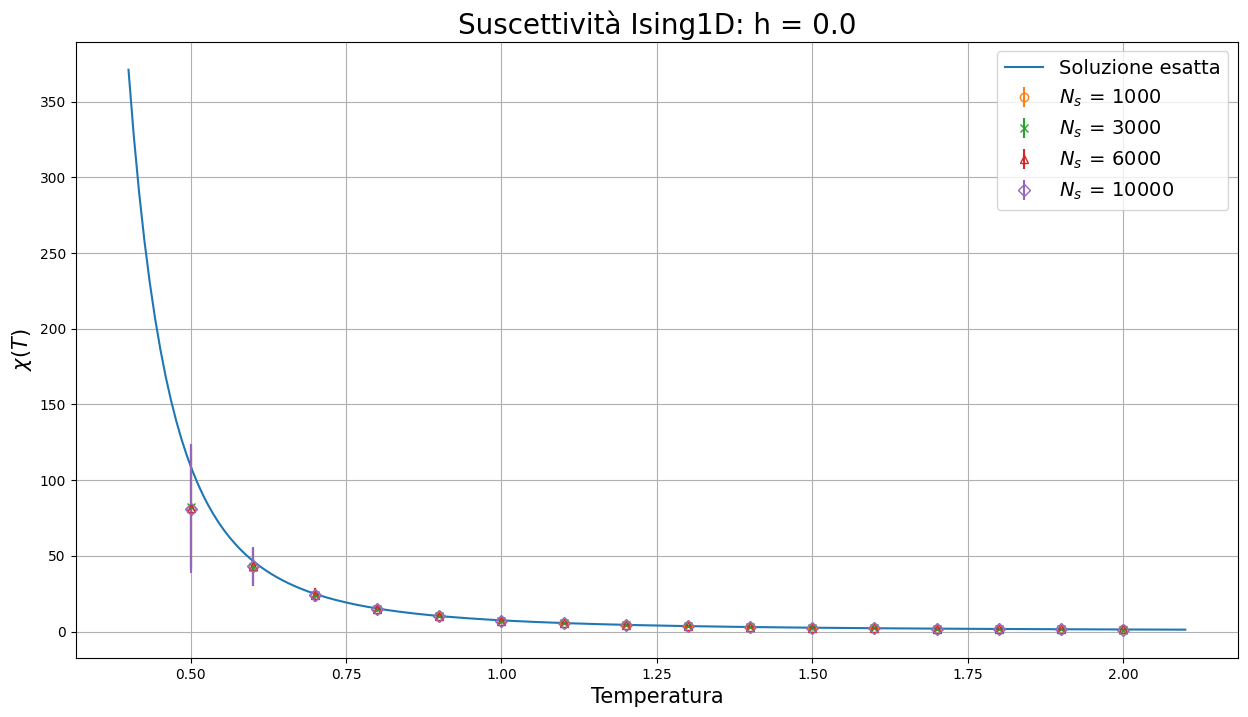
\includegraphics[width=\textwidth]{Immagini/simIsing1D/chi_h0.0.png}
    \caption{Suscettività modello di Ising 1D: h = 0.0.}
    \label{fig: chi_Ising1D_h0.0}
\end{figure}

\begin{figure}[H]
    \centering
    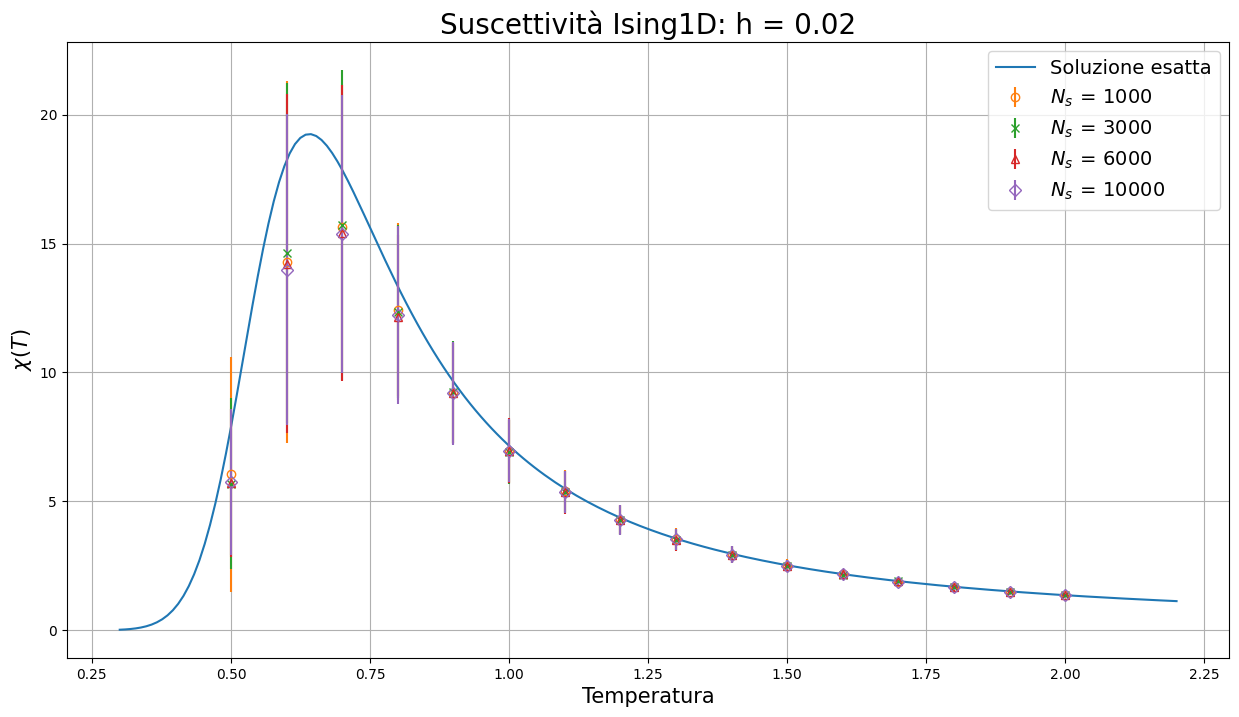
\includegraphics[width=\textwidth]{Immagini/simIsing1D/chi_h0.02.png}
    \caption{Suscettività modello di Ising 1D: h = 0.02.}
    \label{fig: chi_Ising1D_h0.0}
\end{figure}

\begin{figure}[H]
    \centering
    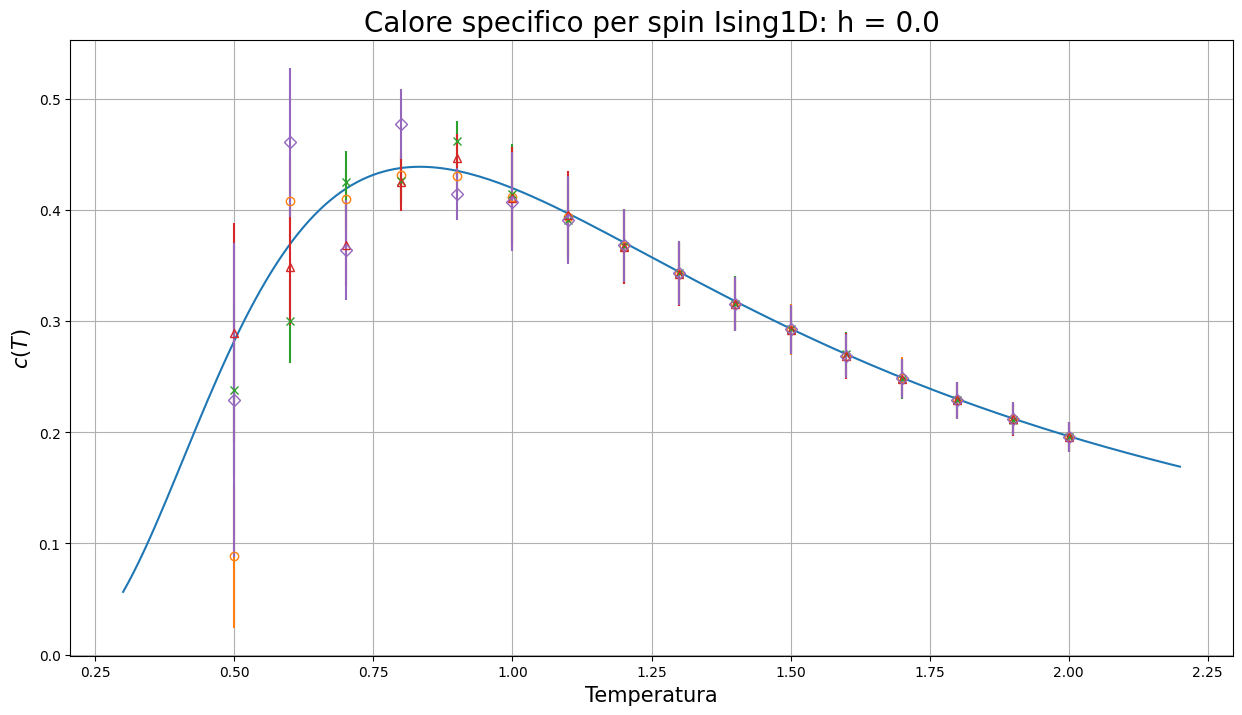
\includegraphics[width=\textwidth]{Immagini/simIsing1D/cp_h0.0.png}
    \caption{Calore specifico modello di Ising 1D: h = 0.0.}
    \label{fig: cp_Ising1D_h0.0}
\end{figure}

\begin{figure}[H]
    \centering
    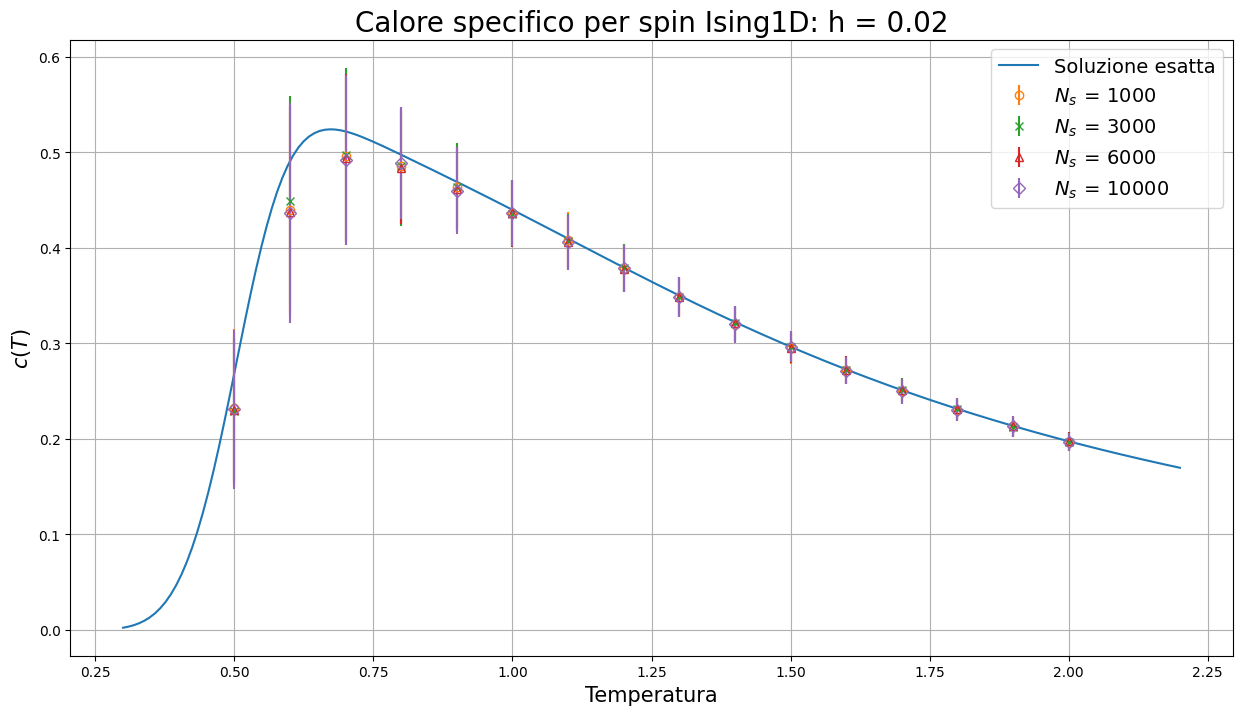
\includegraphics[width=\textwidth]{Immagini/simIsing1D/cp_h0.02.png}
    \caption{Calore specifico modello di Ising 1D: h = 0.02.}
    \label{fig: cp_Ising1D_h0.0}
\end{figure}